\section{Formación de imágenes satelitales}
\subsection{Partes de una imagen}

\begin{frame}{}
  \begin{figure}
    \centering
    \movie[width = 0.8\textwidth,loop,autostart]{\centering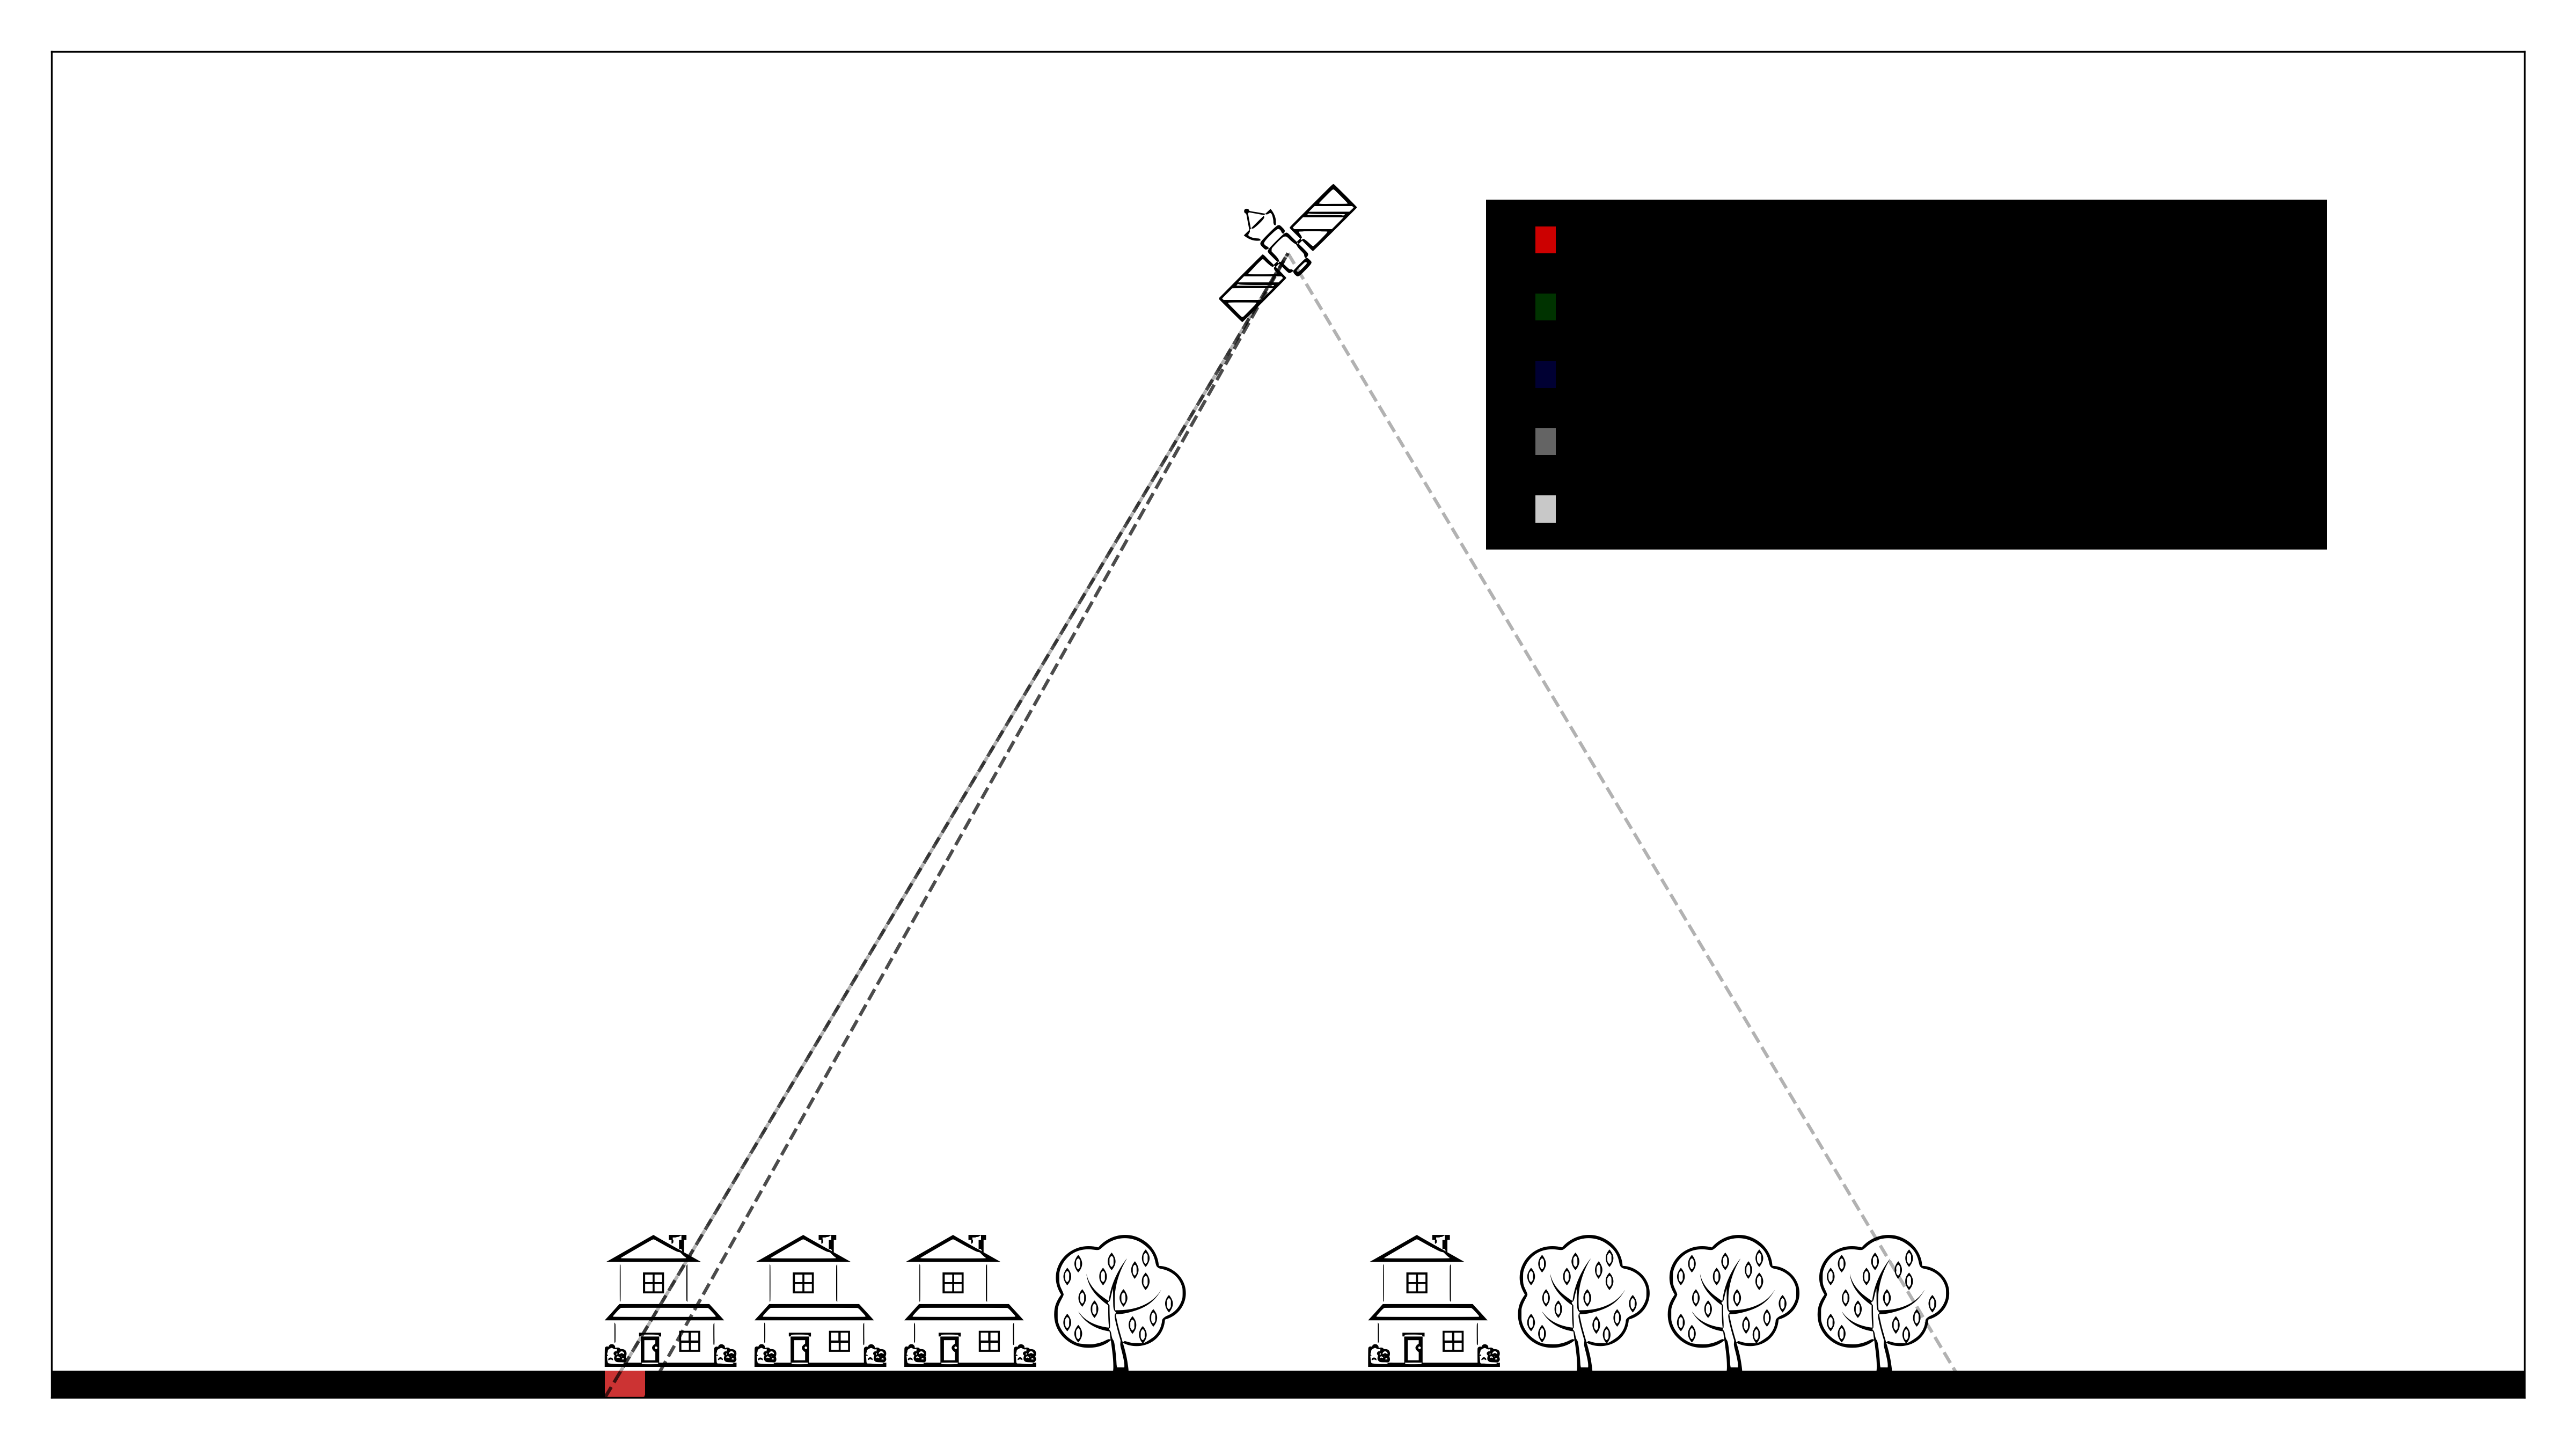
\includegraphics[width=0.8\textwidth]{fig:fimagen.png}}{./figs/fig:fimagen.mp4}
    \caption{Formación de una imagen.}
    \label{}
  \end{figure}
\end{frame}
% modificar el video, no me cierra nada, es bastante confuso, o mejorar o cambiar.
%--- Next Frame ---%

\begin{frame}{}
\begin{block}{Píxel}
  Un píxel es el mínimo elemento de una imagen. Cada píxel tiene un único valor numérico.
\end{block}\pause
\begin{block}{Banda}
  Una banda es un agrupamiento de píxeles en dos dimensiones. Una banda puede estar asociada a una longitud de onda específica o a una operación matemática.
\end{block}
\end{frame}
%--- Next Frame ---%


\begin{frame}{}
  \begin{block}{Imagen}
    En general vamos a hablar de una imagen, o un raster, como el conjunto de bandas.
  \end{block}
\end{frame}
%--- Next Frame ---%

\subsection{Resolución espectral y radiométrica}

\begin{frame}{}
  \begin{block}{Radiometría}
    Resolución radiométrica
  \end{block}
\end{frame}
%--- Next Frame ---%

\begin{frame}{}
  \begin{block}{8 bits}
   \begin{equation}
            2^8 = 0-255
        \end{equation}
  \end{block}
\end{frame}

%--- Next Frame ---%

\begin{frame}{}
  \begin{figure}
    \centering
    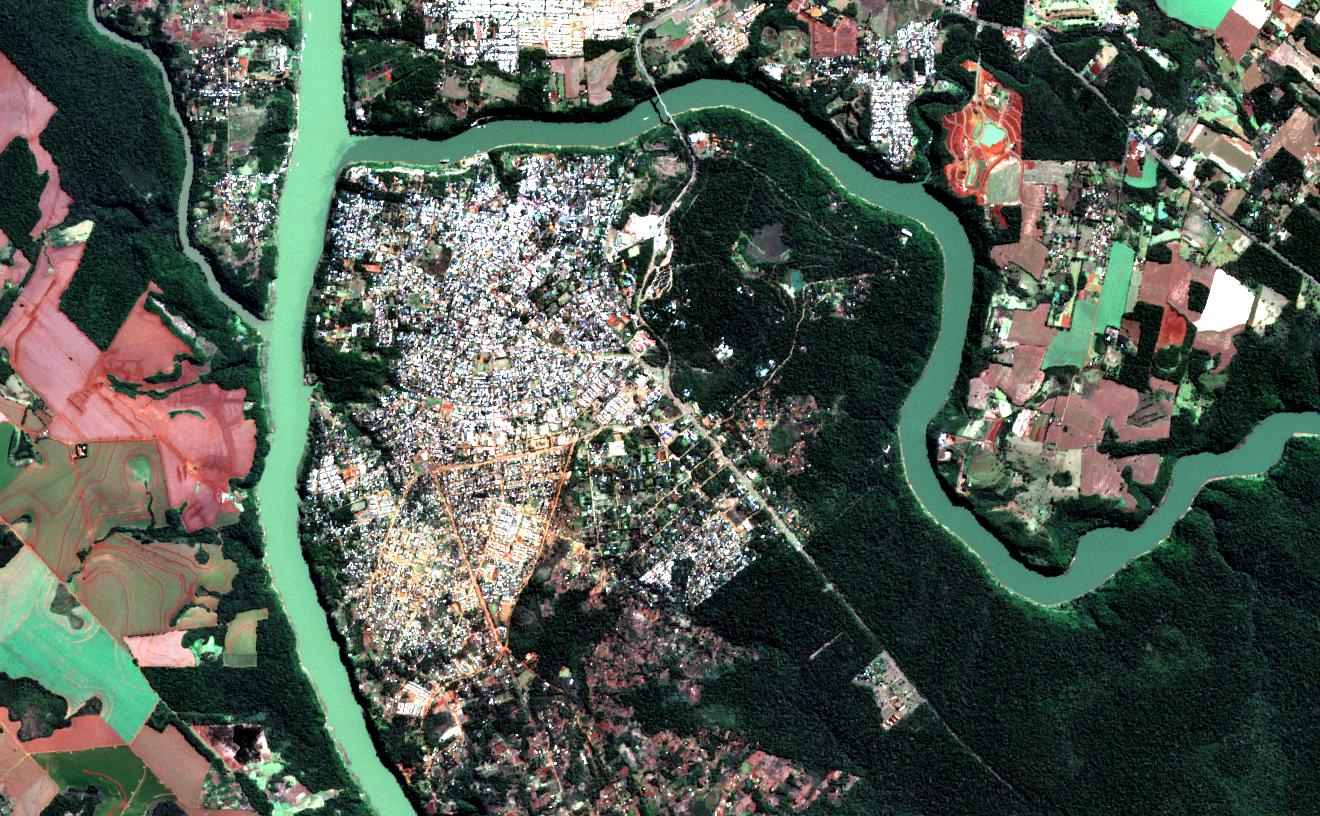
\includegraphics[width=0.7\textwidth]{fig:8bit.jpg}
    \caption{Imagen con resolución radiométrica de 8bit.}
    \label{}
  \end{figure}
\end{frame}
%--- Next Frame ---%


\begin{frame}{}
  \begin{block}{4 bits}
   \begin{equation}
            2^4 = 0-15
        \end{equation}
  \end{block}
\end{frame}

%--- Next Frame ---%

\begin{frame}{}
  \begin{figure}
    \centering
    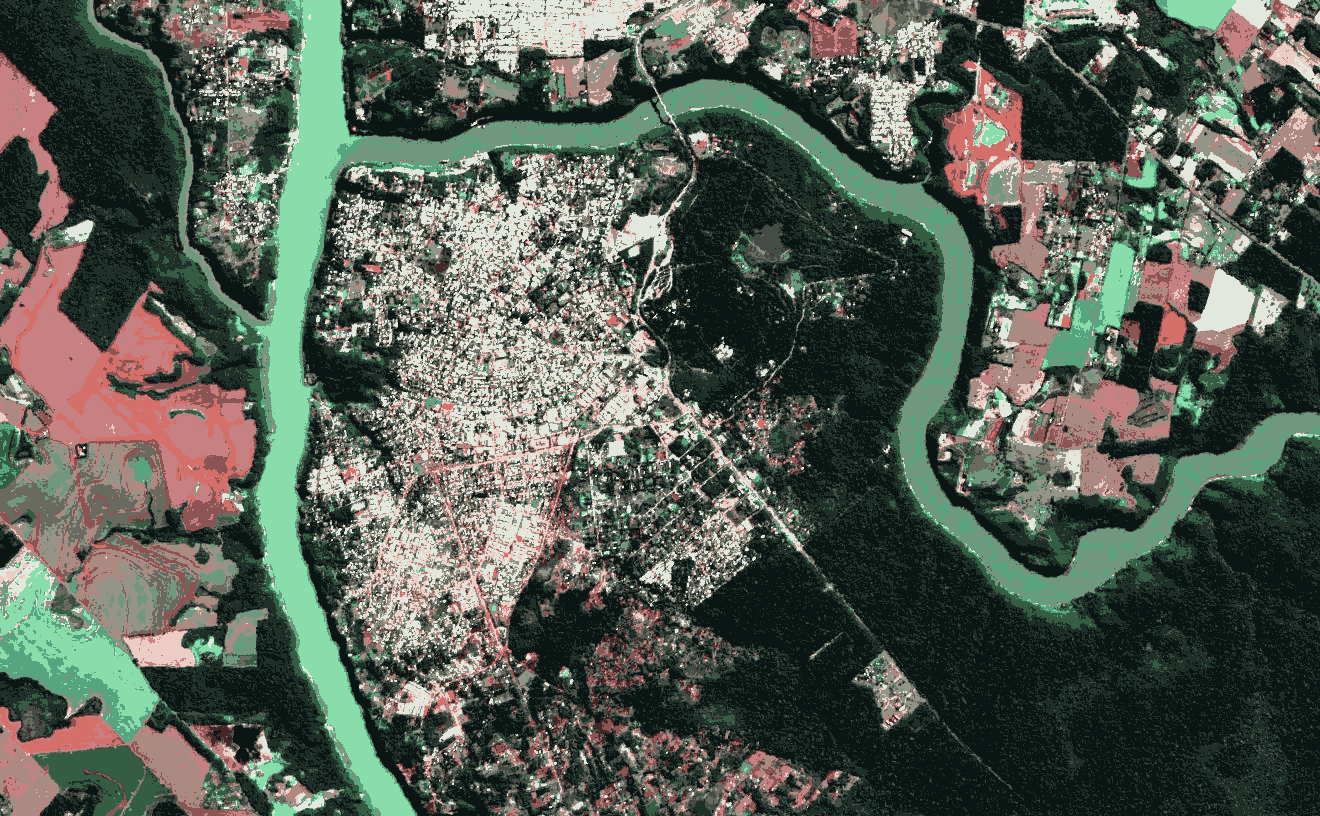
\includegraphics[width=0.7\textwidth]{fig:4bit.jpg}
    \caption{Imagen con resolución radiométrica de 4bit.}
    \label{}
  \end{figure}
\end{frame}
%--- Next Frame ---%


\begin{frame}{}
  \begin{block}{2 bits}
   \begin{equation}
            2^2 = 0-3
        \end{equation}
  \end{block}
\end{frame}

%--- Next Frame ---%

\begin{frame}{}
  \begin{figure}
    \centering
    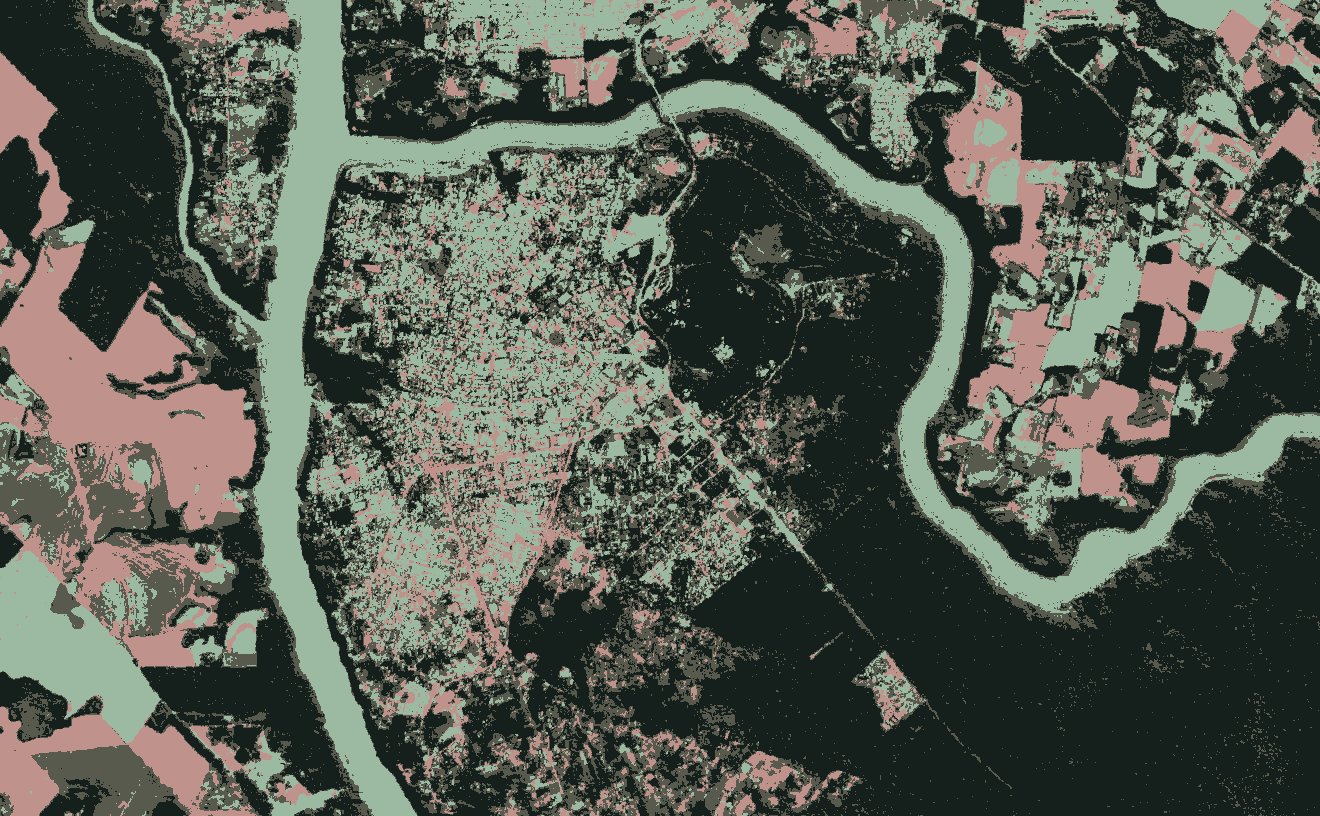
\includegraphics[width=0.7\textwidth]{fig:2bit.jpg}
    \caption{Imagen con resolución radiométrica de 2bit.}
    \label{}
  \end{figure}
\end{frame}
%--- Next Frame ---%



%--- Next Frame ---%

\begin{frame}{}
  \begin{block}{1 bits}
   \begin{equation}
            2^2 = 0-1
        \end{equation}
  \end{block}
\end{frame}

%--- Next Frame ---%

\begin{frame}{}
  \begin{figure}
    \centering
    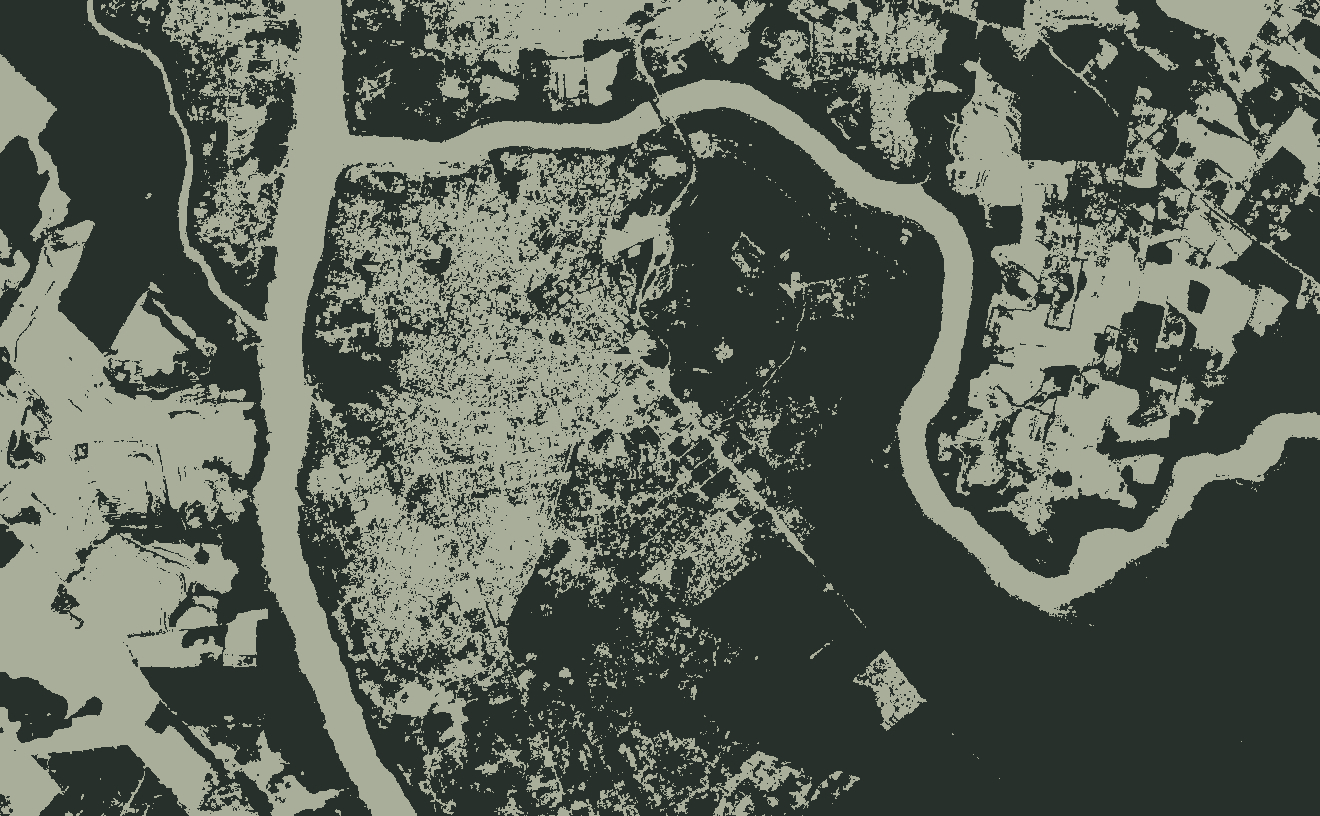
\includegraphics[width=0.7\textwidth]{fig:1bit.jpg}
    \caption{Imagen con resolución radiométrica de 1bit.}
    \label{}
  \end{figure}
\end{frame}
%--- Next Frame ---%



\begin{frame}{}
    \begin{block}{Definición}
        En la capacidad de distinguir cambios en la radiancia que proviene de un píxel y como ésta se cuantifica.
    \end{block}
\end{frame}
%--- Next Frame ---%

\begin{frame}{}
  \begin{figure}
    \centering
    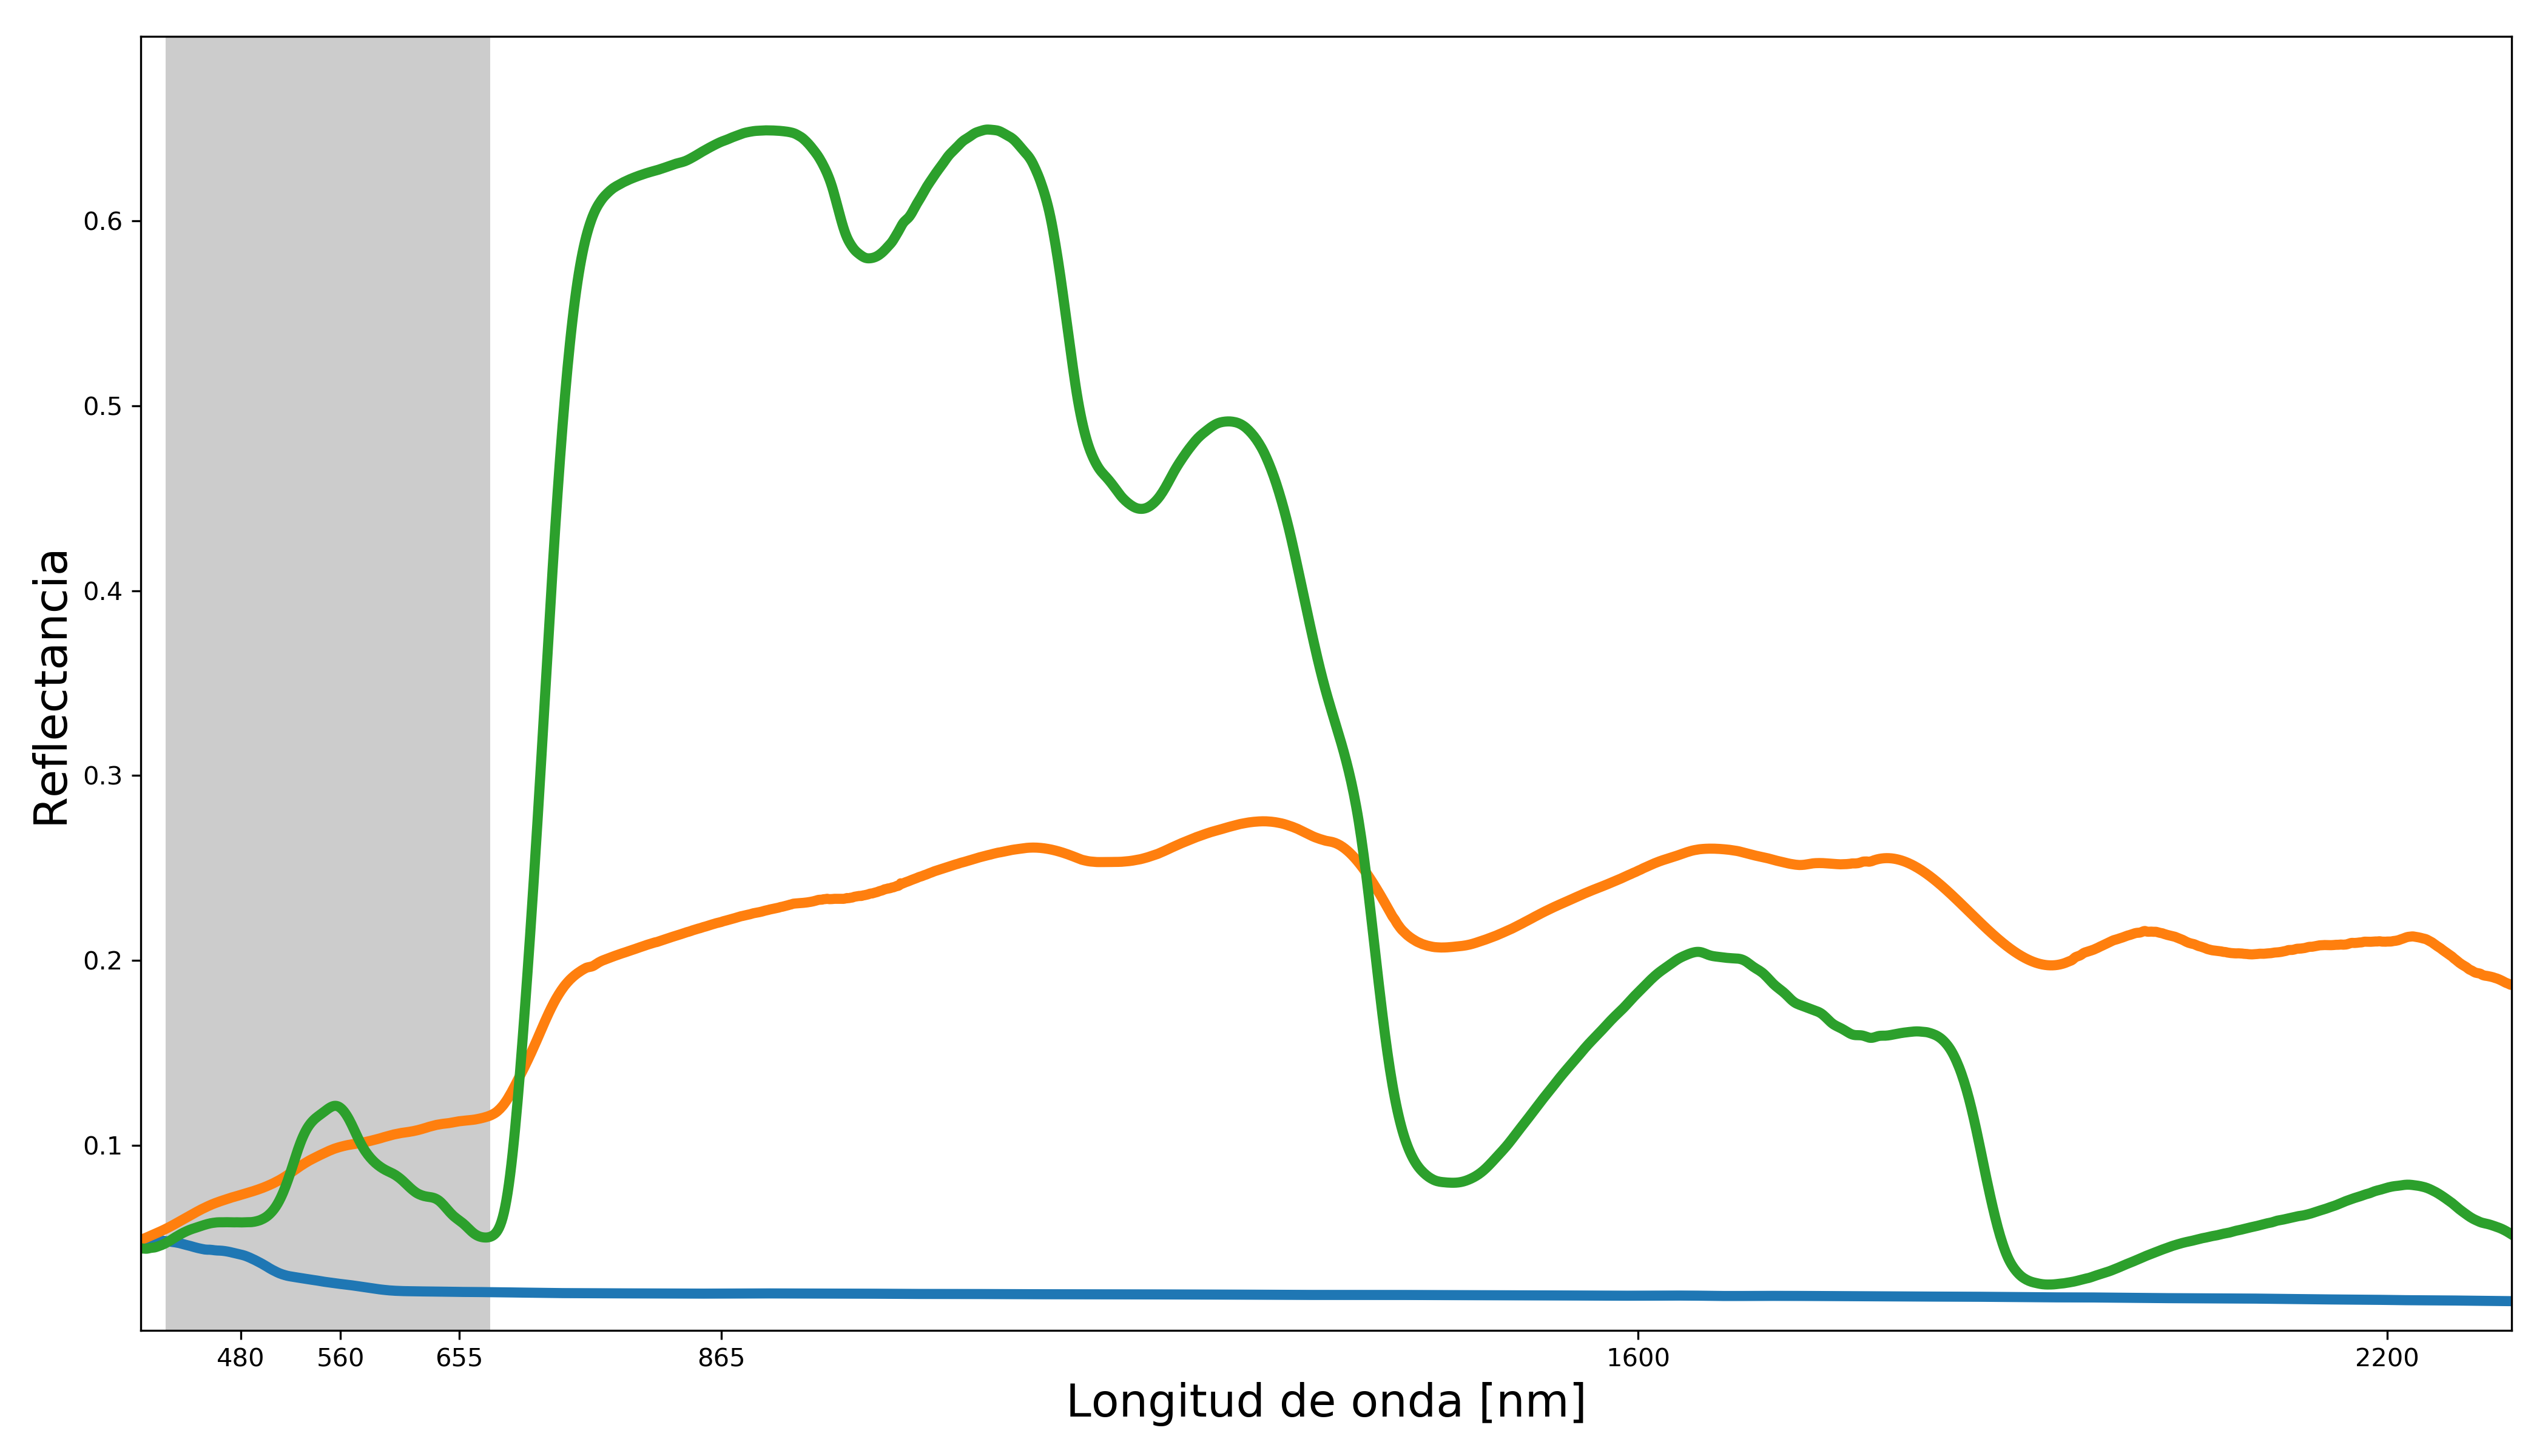
\includegraphics[width=0.8\textwidth]{fig:eslo.png}
    \caption{Resolución espectral sobre la firma espectral.}
    \label{}
  \end{figure}
\end{frame}
%--- Next Frame ---%

\begin{frame}{}
  \begin{figure}
    \centering
    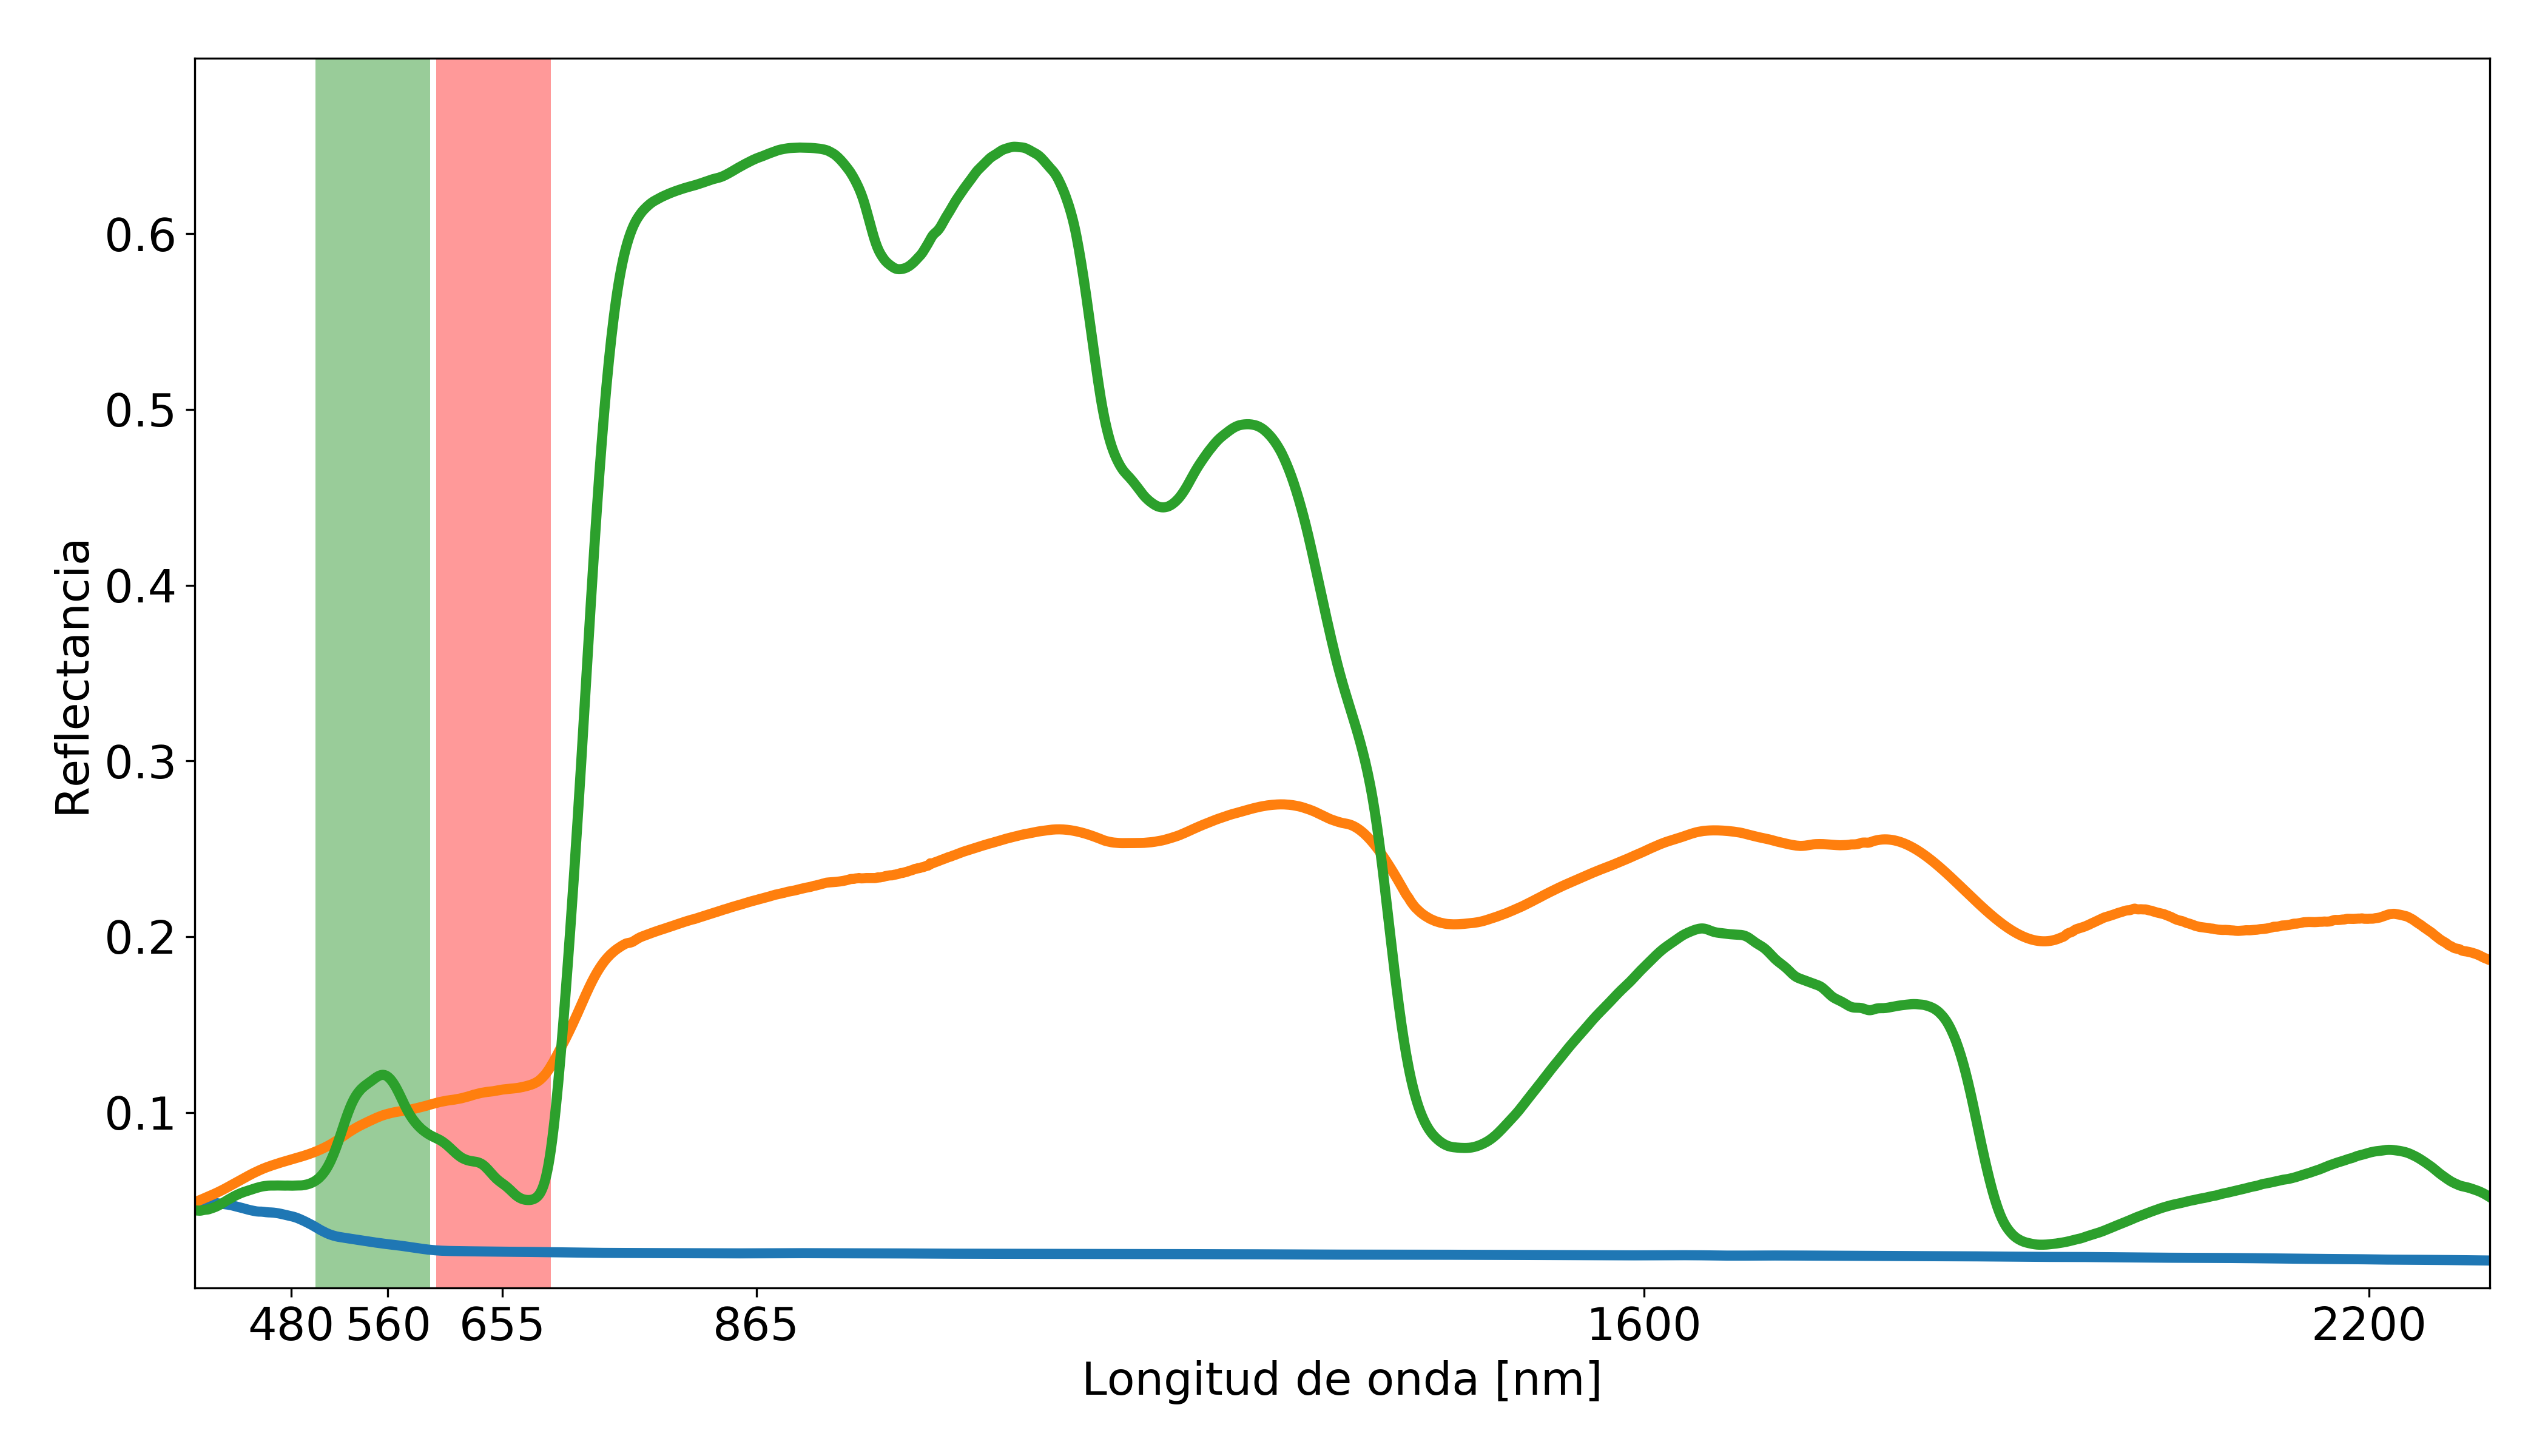
\includegraphics[width=0.8\textwidth]{fig:eshi.png}
    \caption{Resolución espectral sobre la firma espectral.}
    \label{}
  \end{figure}
\end{frame}
%--- Next Frame ---%

\begin{frame}{}
    \begin{block}{Definición}
        Es la capacidad del sensor de distinguir regiones del espectro electromagnético.
    \end{block}
\end{frame}
%--- Next Frame ---%

%\subsection{Proyección sobre el terreno}

%\begin{frame}{}
%  \begin{figure}
%    \centering
    %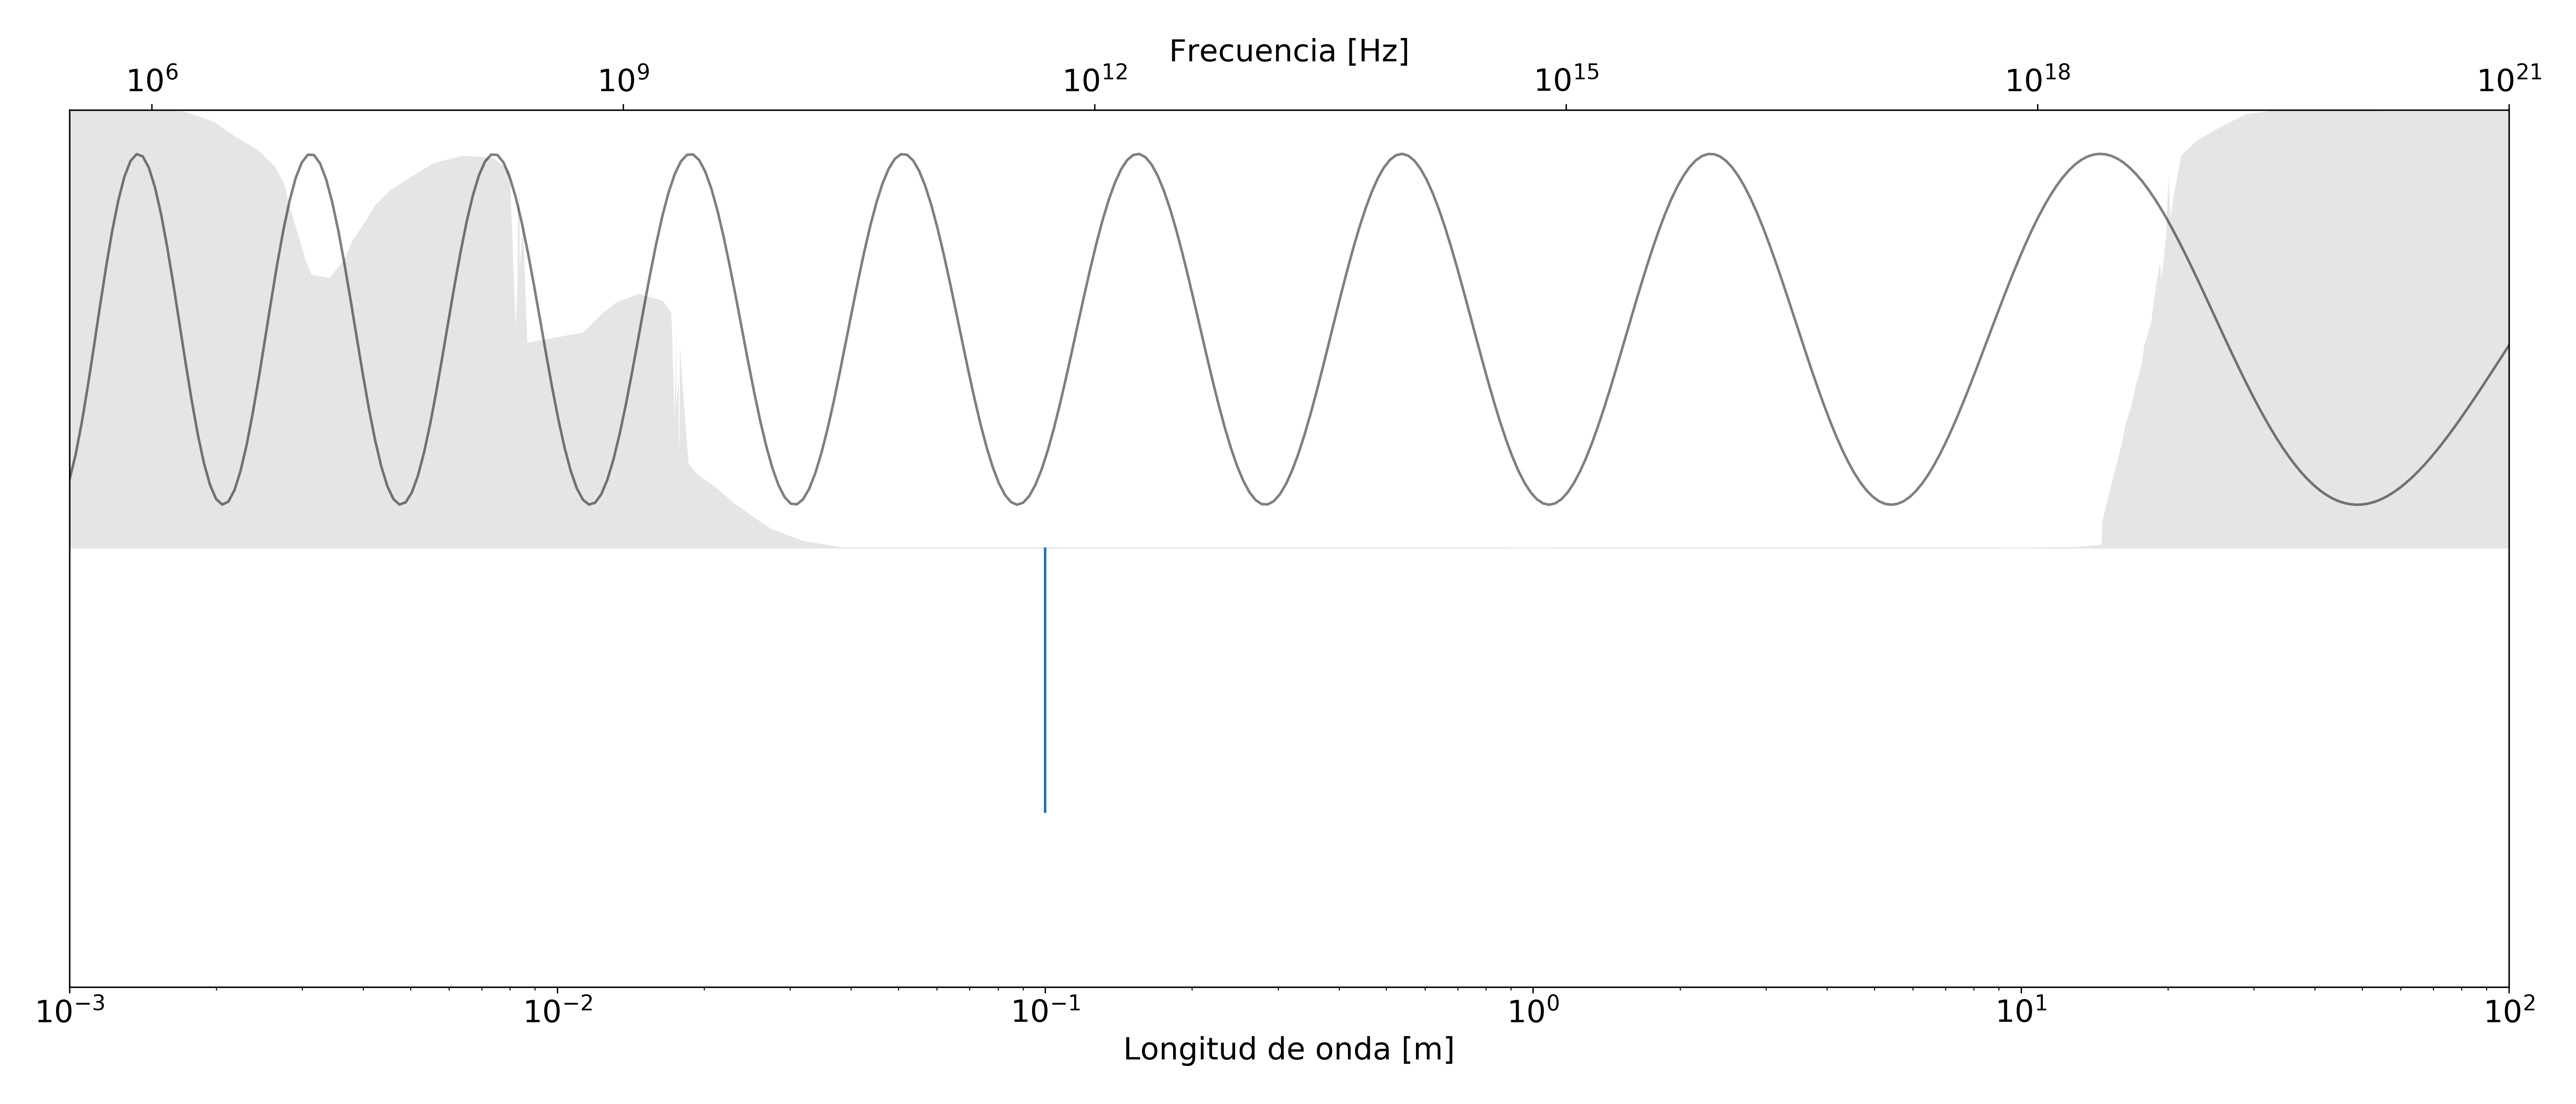
\includegraphics[width=\textwidth]{fig:espectro.png}
%    \caption{Asignación de coordenadas a píxeles.}
%    \label{}
%  \end{figure}
%\end{frame}
%--- Next Frame ---%

%\begin{frame}{}
%  \begin{figure}
%    \centering
    %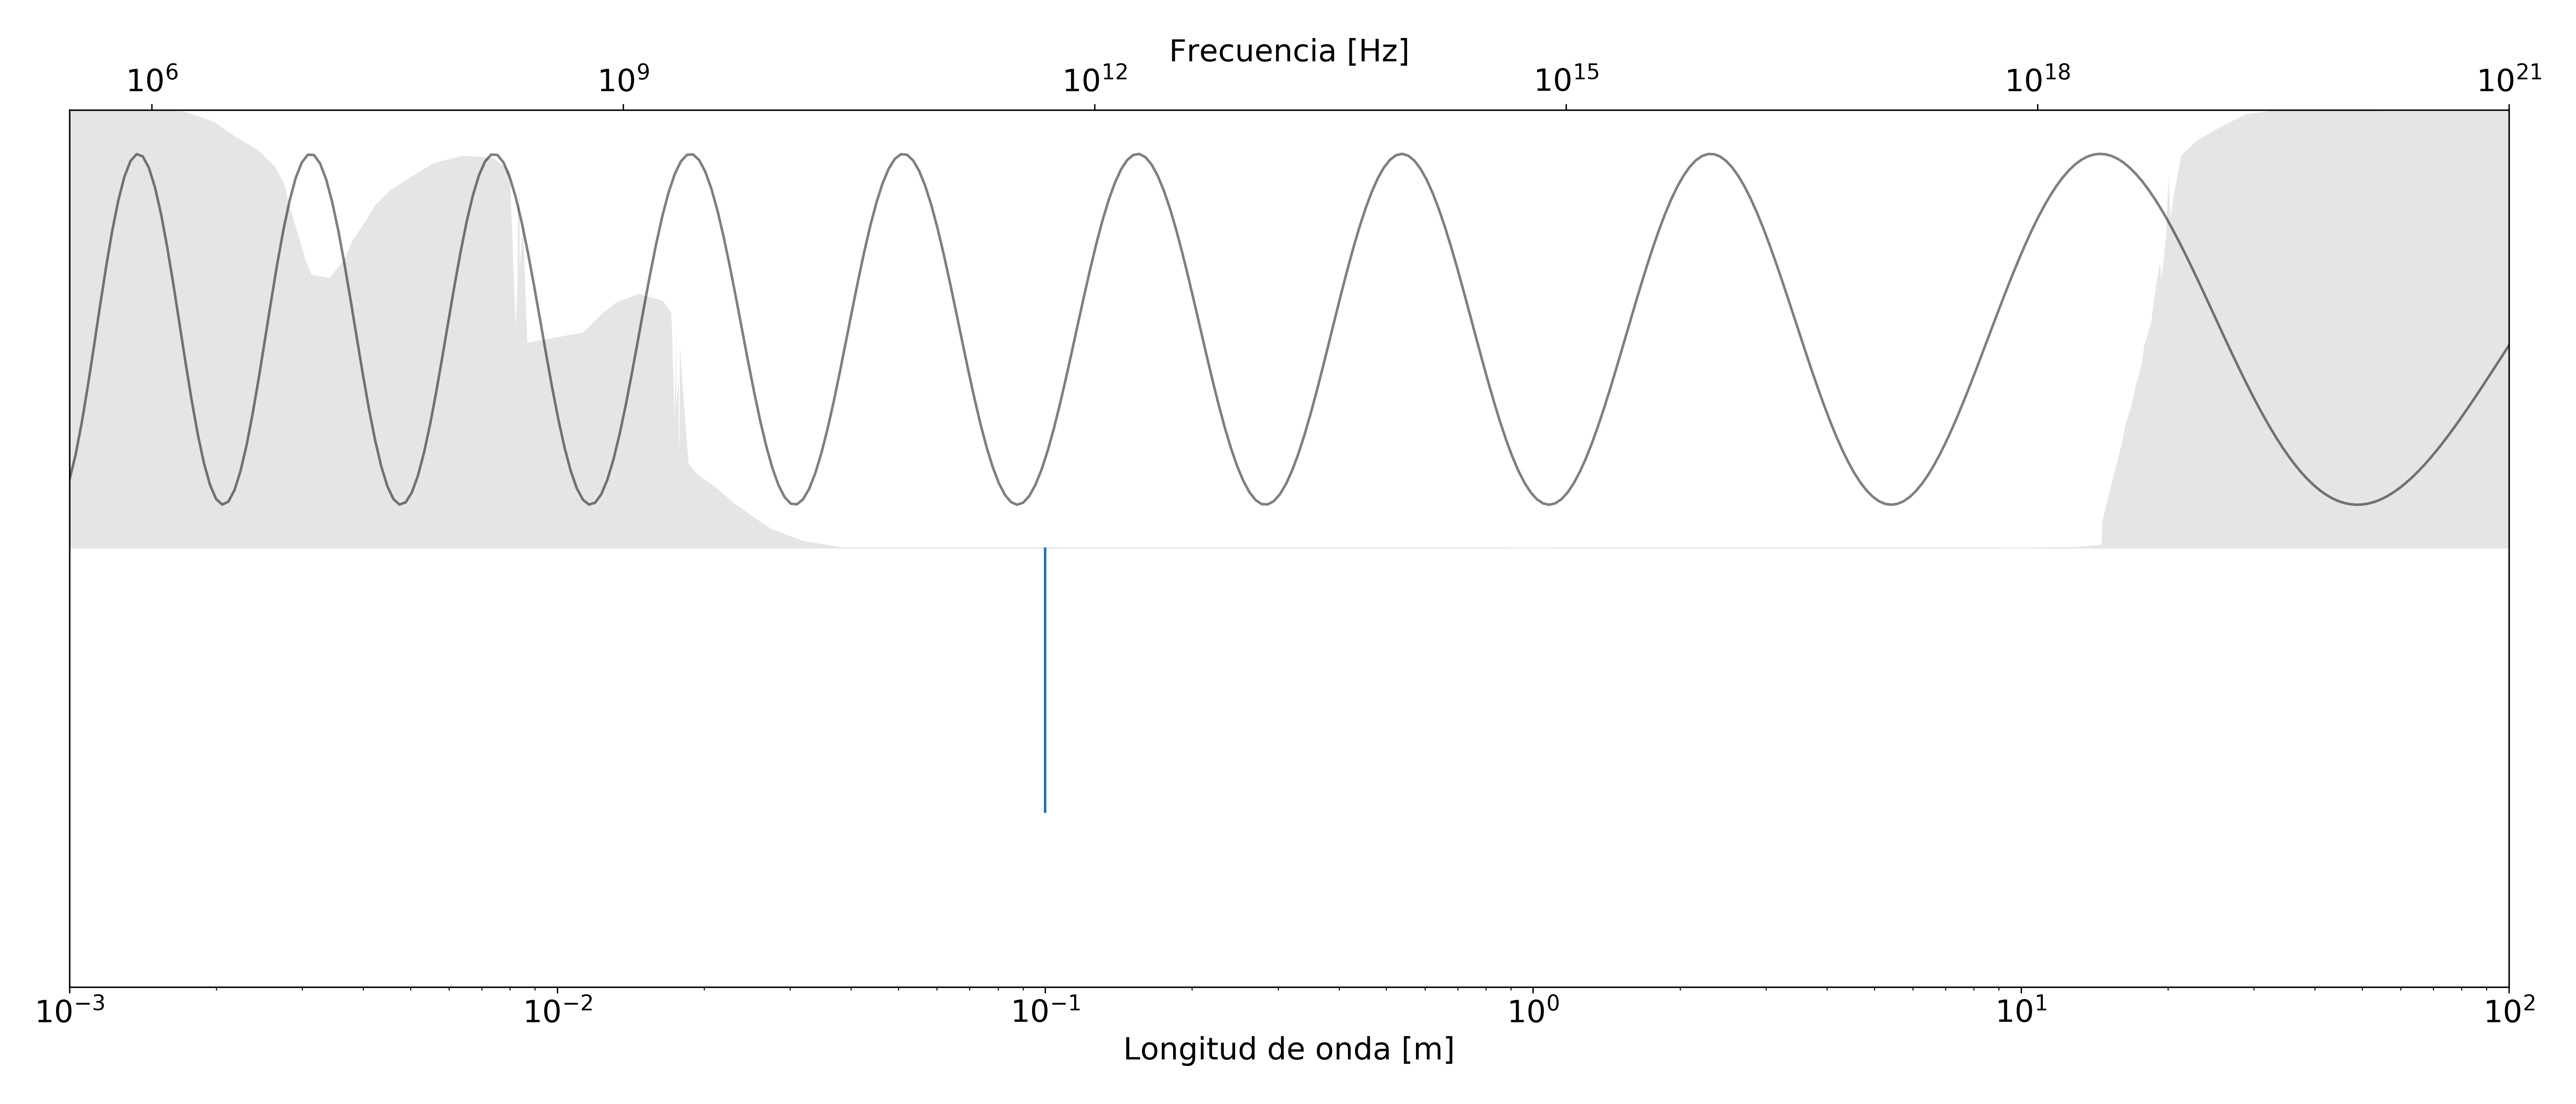
\includegraphics[width=\textwidth]{fig:espectro.png}
%    \caption{Proyección de una esfera en un plano.}
%    \label{}
%  \end{figure}
%\end{frame}
%--- Next Frame ---%

%\begin{frame}{}
%  \begin{figure}
%    \centering
    %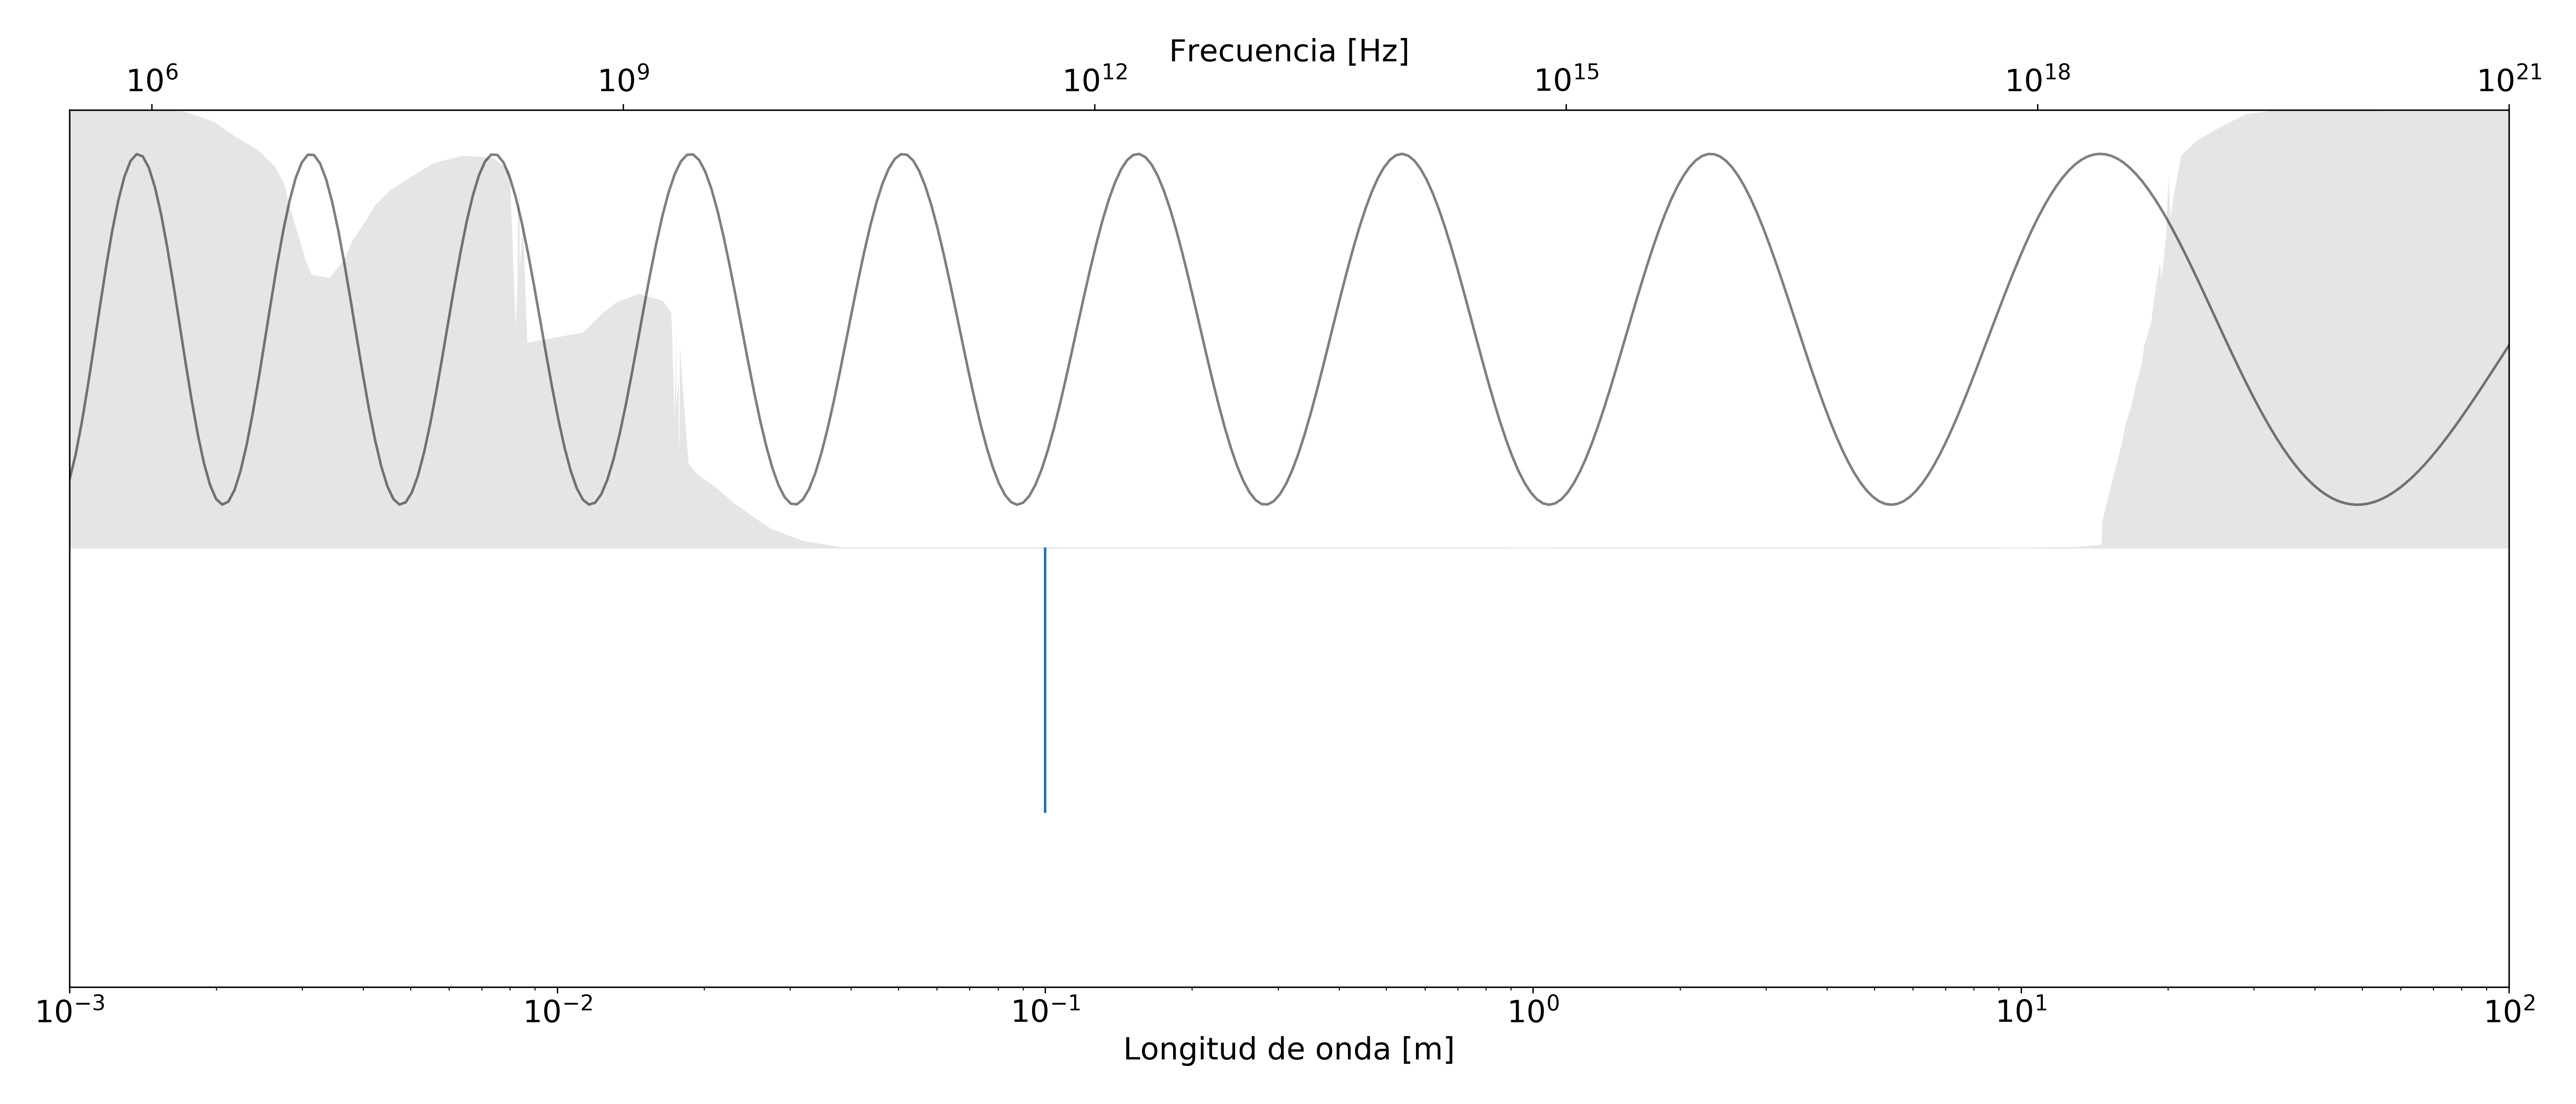
\includegraphics[width=\textwidth]{fig:espectro.png}
%    \caption{Métodos de interpolación.}
%    \label{}
%  \end{figure}
%\end{frame}
%--- Next Frame ---%

%\begin{frame}{}
%  \begin{figure}
%    \centering
%    %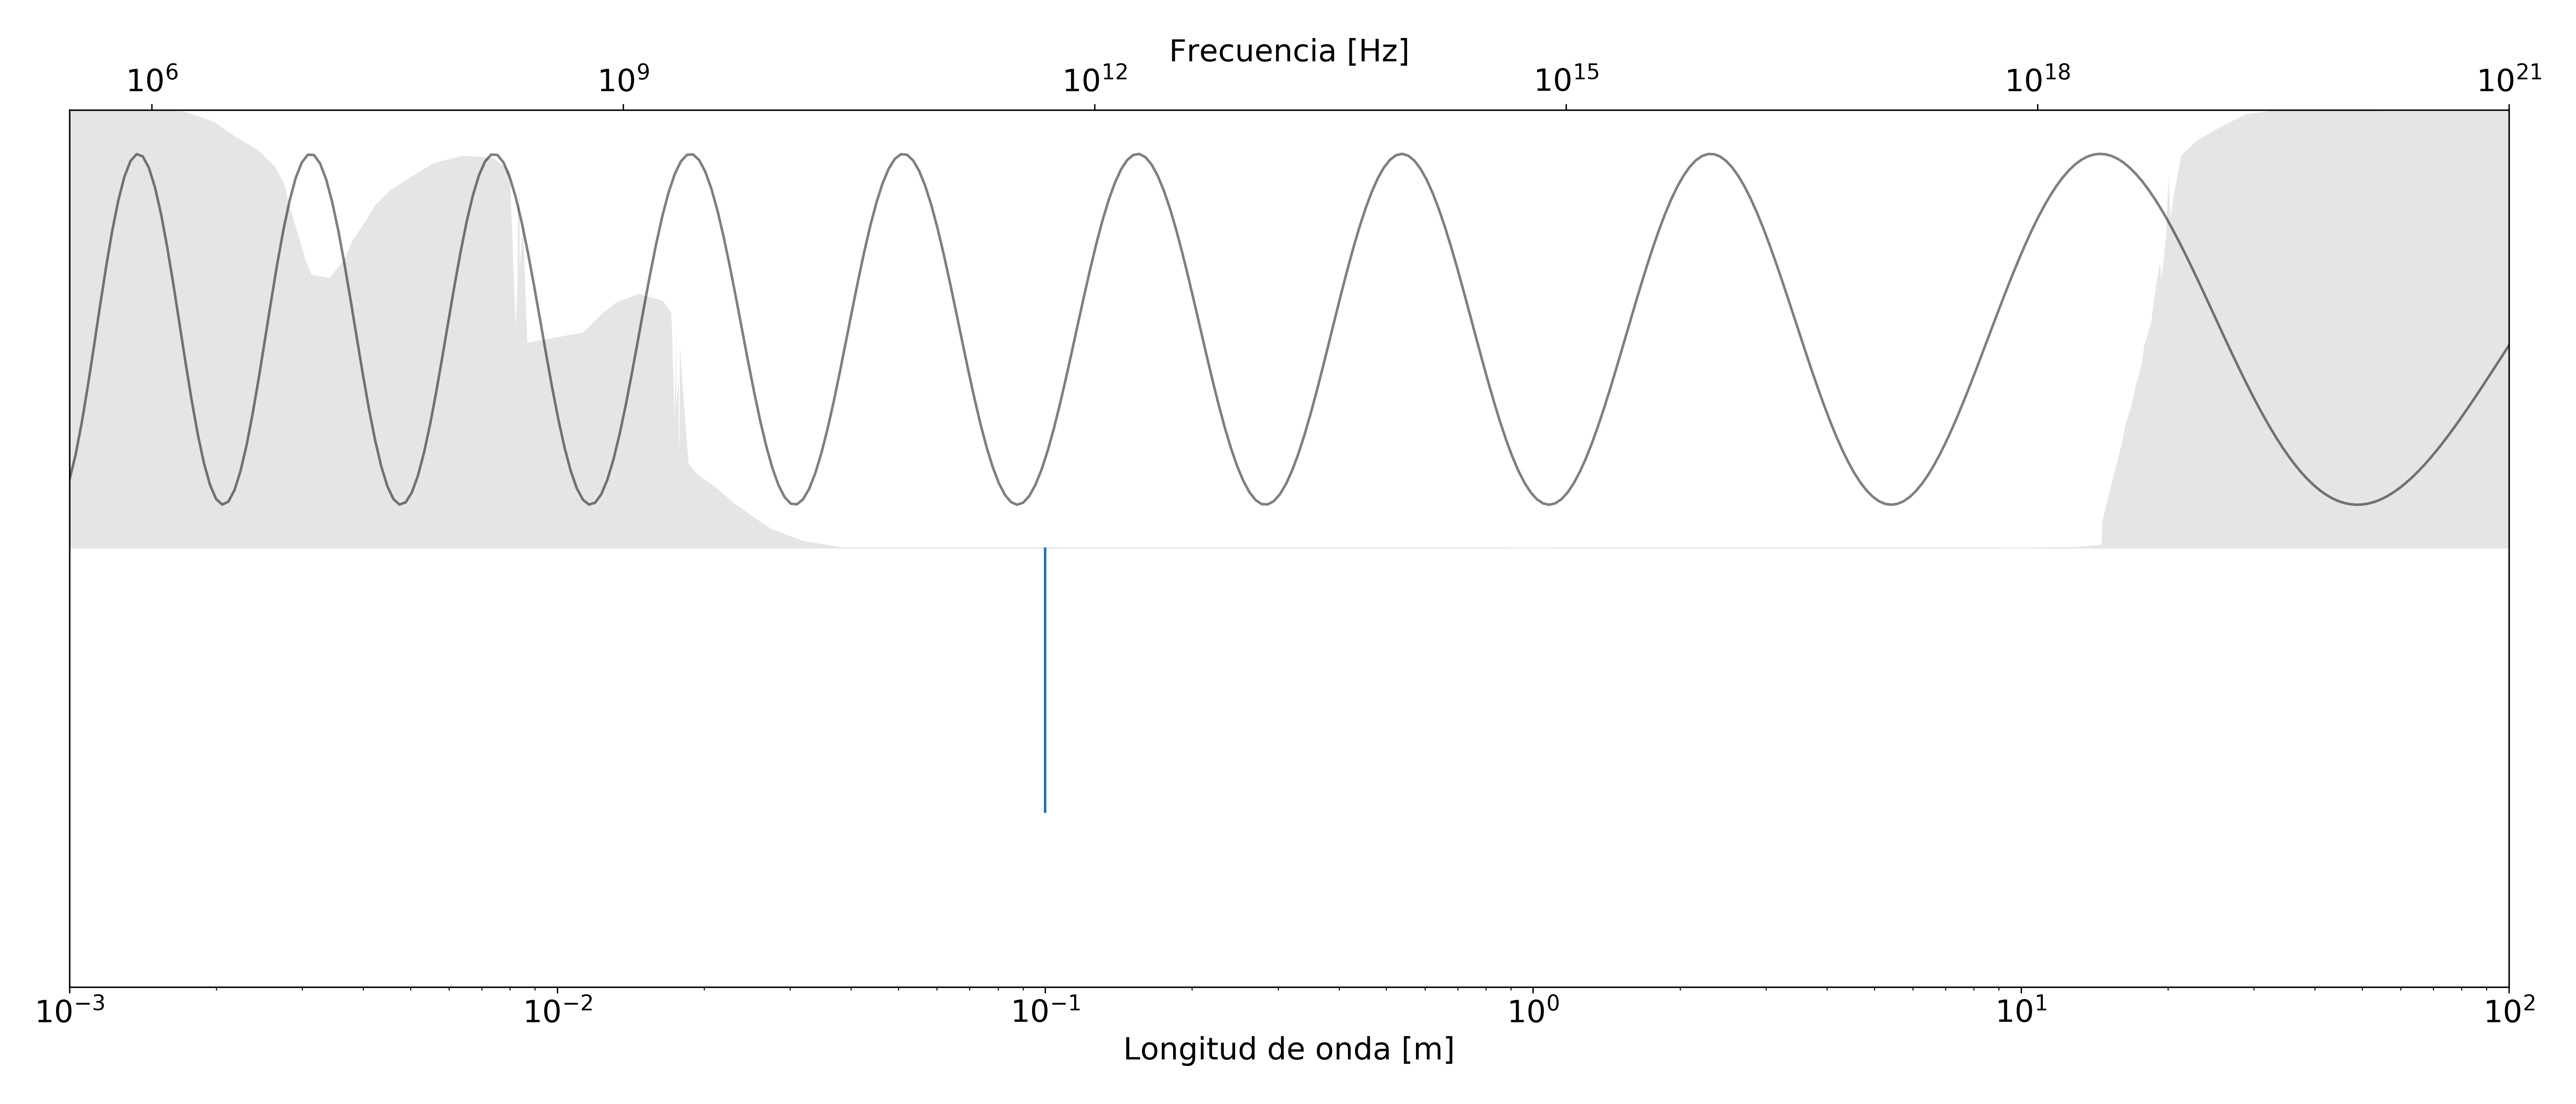
\includegraphics[width=\textwidth]{fig:espectro.png}
%    \caption{Tipos de proyecciones.}
%    \label{}
%  \end{figure}
%\end{frame}
%--- Next Frame ---%



\gracias
%--- Next Frame ---%
